\documentclass[a4paper,10pt]{article}

\usepackage[utf8]{inputenc}
\usepackage{t1enc}
\usepackage[spanish]{babel}
\usepackage[pdftex,usenames,dvipsnames]{color}
\usepackage[pdftex]{graphicx}
\usepackage{amsmath}
\usepackage{hyperref}
\usepackage{amsfonts}
\usepackage{amssymb}
\usepackage{listings}
\lstset{language=C}
\lstset{showstringspaces=false}
\lstset{basicstyle=\ttfamily,}

\begin{document}


\renewcommand{\lstlistingname}{C\'odigo Fuente}
\lstloadlanguages{Octave} 
\lstdefinelanguage{MyPseudoCode}[]{Octave}{
	deletekeywords={beta,det},
	morekeywords={repmat}
} 
\lstset{
	language=MyPseudoCode,
	stringstyle=\ttfamily,
	showstringspaces = false,
	basicstyle=\footnotesize\ttfamily,
	commentstyle=\color{gray},
	keywordstyle=\bfseries,
	numbers=left,
	numberstyle=\ttfamily\footnotesize,
	stepnumber=1,                   
	framexleftmargin=0.20cm,
	numbersep=0.37cm,              
	backgroundcolor=\color{white},
	showspaces=false,
	showtabs=false,
	frame=l,
	tabsize=4,
	captionpos=b,               
	breaklines=true,             
	breakatwhitespace=false,      
	mathescape=true
}
\begin{titlepage}
        \thispagestyle{empty}
        \begin{center}
                
\includegraphics{./images/itba.jpg}
                \vfill
                \Huge{Sistemas Operativos}\\
                \vspace{1cm}
                \huge{Trabajo Práctico Especial}\\
        \end{center}
        \vspace{2cm}
        \large{
                \begin{tabular}{lcrc}
                        \textbf{Alvaro Crespo} & & 50758 & \ \ \texttt{acrespo@alu.itba.edu.ar}\\
                        \textbf{Juan Pablo Civile} & & 50453 & \ \ \texttt{jcivile@alu.itba.edu.ar}\\
                        \textbf{Darío Susnisky} & & 50592 & \ \ \texttt{dsusnisk@alu.itba.edu.ar}\\
                        \\ 
                \end{tabular}
        }
        \vfill
        \flushright{24 de Octubre del 2011}
\end{titlepage}

\setcounter{page}{1}

\tableofcontents
\newpage
\section{Introducción}
El trabajo práctico consistía en la extensión del sistema operativo armado en la materia arquitectura de las 
computadoras. Este debia ser modificado de modo tal que esta nueva versión soporte procesamiento multitareas
 (inclusive con más de una técnica de \textit{scheduling}), soporte de acceso a disco rígido y un \textit{file system}
 no tan básico con varios detalles interesantes (soporte de usuarios y grupos, \textit{FIFO's}, entre otros).

\newpage
\section{Breve resumen de la vieja versión de Arqvengers OS}
El trabajo práctico fue comenzado tomando como base el trabajo hecho en la materia Arquitectura de las Computadoras.
 Este trabajo contaba con un sistema operativo booteable que contaba con soporte para \textit{drivers} de
  teclado y de video facilitando varias consolas en donde podían ejecutarse distintos comandos. 
  A un nivel más bajo, contabamos con una rudimentaria e incompleta librería de C así como una interfaz para realizar
  llamadas a sistema.
\newpage
\section{Procesos}

\subsection{Estructura de un proceso}
La estructura de proceso contiene toda la informacion necesaria para ejecutar el proceso y atender llamadas al sistema.
Basicamente la informacion que contiene es:
\begin{itemize}
\item Contexto de ejecucion
\item Padre
\item Usuario y grupo
\item Archivos abiertos
\item Estado de scheduling
\end{itemize}

El contexto de ejecucion es la parte fundamental de la estructura.
Este contiene la memoria que es el stack y el heap del proceso.
Tambien contiene una referencia al punto de entrada del proceso, y los argumentos pasados al momento de creacion.

Para permitir la interaccion con el file system, el proceso tiene una tabla de que archivos tiene abiertos.
Ademas, el usuario que lo ejecuto, que es necesario para verificar permisos.

\subsubsection{Stack inicial}
Una parte muy importante, y delicada, de la creacion de un proceso nuevo es la inicializacion del stack del proceso.
Es necesario asegurar que en el momento que el scheduler cambie al contexto del proceso por primera vez, este pueda salir de la interrupcion que genero el cambio.
Tambien se asegura que cuando se retorna del punto de entrada del proceso, se llama a \textit{exit} para que este termine con exito.

    \subsection{Scheduling}
        
        \subsubsection{Interfaz}
        En una primera instancia, se creó una interfaz a la cual todas las implementaciones del \textit{scheduler} que se hicieran
	deberían atenerse. Para una vista detallada de dicha interfaz dirigigirse al archivo \textit{src/system/scheduler.h}.

        \subsubsection{Implementación general}
	Luego de algunas primeras y simples implementaciones del \textit{scheduler} nos dimos cuenta que ambas estrategias que 
	implementaríamos serían prácticamente iguales: solo se diferenciaban en la forma en que se escogía al siguiente proceso
	para darle tiempo de ejecución. 

	Esto pudo lograrse a nuestra estructura de datos \textit{ProcessQueue} la cual se adaptó con facilidad a ambas estrategias.

	Cabe destacar en este punto también, que para implementar procesos dormidos (\textit{sleep}) hubo que implementar otra estructura
	de datos, \textit{SleepList}. Esta estructura de datos no es otra cosa que la conocida \textit{Delta Queue}, utlizada para resolver 
	esta clase de problemas.

        \subsubsection{Primera estrategia: Round Robin}
        Como primera estrategia de \textit{scheduling} se decidió implementar una simple estrategia de \textit{Round Robin}.
        Esto es, los períodos de tiempo de uso de CPU (\textit{time slices}) son asignados a los procesos en porciones 
        equivalentes y en orden circular, sin hacer uso de un sistema de prioridades. Este estrategia, además de ser muy 
        fácil de implementar, asegura la provisión de tiempo de CPU a todos los procesos (\textit{starvation free}).

	En nuestra implementación, utilizando la \textit{ProcessQueue} lo único que se hace es desencolar el siguiente proceso 
	de la cola y encolar al final de ella al proceso que estaba ejecutando.

        \subsubsection{Segunda estrategia: Algoritmo basado en prioridades}
        Para nuestra segunda estrategia, y siguiendo con la consigna del trabajo, implementamos un sistema basado en 
        prioridades. El algoritmo para elegir al siguiente proceso al que se le asignara un \textit{time slice} utiliza
        2 parámetros: la prioridad de un proceso y su "prioridad acumulada". El mismo tiene la siguiente forma:

        En un primer momento todos los procesos tienen prioridad acumulada 0. Al momento de elegir el siguiente proceso
        se le suman a las "prioridades acumuladas", las prioridades de cada proceso. Luego, se elige como siguiente 
        proceso al que tenga mayor "prioridad acumulada" y a dicho proceso se le reinicia su "prioridad acumulada" a 0.
        El resto de los proceso mantienen s'us "prioridades acumuladas" para el siguiente turno. 

        En cada momento de elección, se repite ese procedimiento. Este simple algoritmo, asegura que los procesos con 
        mayor prioridad recibirán mayor tiempo de ejecución que los de menor prioridad, y que, tarde o temprano, todos
        podrán ejecutarse.

\subsection{Multiples Terminales}
Para el soporte de varias terminales, optamos por crear un proceso \textit{tty}, como mediador entre las \textit{shells} y el teclado y pantalla.
Este proceso recibe los pedidos de IO de los procesos que deseen escribir a pantalla o leer de teclado.

Una de sus tareas es tener en cuenta que proceso es activo, y por lo tanto, si puede o no leer del teclado.
Si un proceso no activo intenta leer de teclado, se lo bloquea hasta que este estado cambie, o se mate al proceso.
De la misma manera, para escribir a pantalla, se tiene el concepto de terminal activa.
Es responsabilidad de \textit{tty} asegurar que solo se vea el output de la terminal activa, y que ante un cambio de terminal se redibuje la pantalla.

Una de las motivaciones mas importantes para hacer de esto un proceso dedicado, es poder interpretar el input de teclado aun mientras el proceso activo no pida entrada.
Es decir, es posible cambiar entre terminales cuando ningun proceso esta pidiendo input, ya que esta operacion la hace \textit{tty}.

Una particularidad muy importante de \textit{tty} es que es uno de los dos procesos de \textit{kernel}.
Al decir proceo de kernel, significa que corre en el contexto de memoria del kernel, y por lo tanto, puede hacer acceso directo a operaciones del kernel.
Esto resulto ser necesario y muy valioso, por que permite a este proceso acceder a informacion de los procesos, y bloquearlos en caso de ser necesario.
A pesar de esto, en todo otro aspecto se lo trata como un proceso normal.

Una vez inicializado \textit{tty} este crea los procesos de \textit{login}, cada uno en su propia terminal.
Este proceso se encarga de verificar las credenciales del usuario, y en caso de ser correctas, ejecutar el shell para que el usuario pueda utilizar el sistema.
Entonces, cada shell es un proceso independiente, en su propia terminal.

\newpage
\section{Usuarios y grupos}
Alvamaister! GO GO!

\newpage
\section{Driver Ata}
    Se comenzó a implementar un \textit{driver} ATA en modo PIO. Esto significaba que los accesos a disco iban a ser
    por medio de puertos de entrada/salida. Esto hace que el tiempo de ejecución sea considerable pero era un estandar
    confiable y sencillo de implementar.
    El estandar permite acceder a dos discos simultaneamente pero nosotros no vimos la necesidad de implementar el 
    acceso a más de uno.
    
    El primer paso era detectar el disco y obtener ciertos datos del disco en sí. Por suerte, GRUB provee una estructura
    con varios datos del sistema, entre ellos, datos del disco. Trás leer las especificaciones de \textit{multiboot}
    fue relativamente sencillo realizar este trabajo.

    A la hora de elegir el modo de direccionamiento nos encontramos con tres opciones. CHS se vió descartada de forma
    inmediata dado su estado de obsoleta. Luego existian las opciones de LBA 28 y LBA 48 (sus números representan
    la cantidad de bits relevantes utilizados para la dirección). LBA 28 también estaba obsoleto para ciertos discos
    pero era más rapido, más sencillo de implementar y dejaba satisfechas las necesidades de este trabajo.

    Las unidades minimas de lectura y escritura en nuestra implementación son de a sectores, pudiendo ser de a
    varios a la vez. Es un paso escencial poner los datos correctos en los puertos necesarios previo a los accesos, pero
    es aún más interesante la lectura del estado del disco. Esto es necesario para detectar errores en el disco
    y para saber si el disco esta listo para recibir o enviar datos. Es posible que haya que esperar a que el disco
    este listo antes de realizar alguna operación. Hay dos maneras de realizar esta espera, se puede esperar a que una IRQ
    indique que el disco esta listo o se puede consultar el estado del disco hasta que este este listo (\textit{polling}).
    Hacer \textit{polling} puede hacer que se pierda tiempo en un sistema multitareas, pero por otro lado una sola
    consulta de \textit{polling} es más rápida que esperar a una IRQ e implementar \textit{polling} es mucho más sencillo.
    Por esta última razón fue elegida la técnica de \textit{polling}.
\newpage
\section{File System}
    
Una vez implementado el \textit{driver} ATA era posible comenzar a implementar nuestro \textit{file system}.
Dado que nuestra intención era realizar un \textit{file system} persistente debiamos contar con ciertas estructuras
y ciertas especificaciones de como iba a estar representado el mismo en el disco. Luego de hacer un relevamiento
en el tópico decidimos que el implementar un sistema de tipo Ext2 abarcaba todas las caracteristicas que deseabamos
en nuestro sistema. 

Si bien es posible que un sistema Ext2 exceda los requerimientos del trabajo práctico, decidimos que era más seguro seguir este estandar. 
Las herramientas provistas en la distribuciones de Linux para la manipulacion de ext2 probaron ser el mayor beneficio de esta eleccion.
Contar con \textit{fsck} permitio asegurar el correcto funcionamiento de nuestra implementacion.

Una vez terminado el esqueleto que significaba el \textit{file system} se pudo profundizar en el mismo agregando
nuevas funcionalidades, particularmente vamos a hacer hincapie en las consecuencias de aperturas y manejo de
archivos, directorios, FIFO's, links simbolicos, \textit{current working
directory}, permisos del sistema y usuarios y grupos.

A continuación se presentan secciones detalladas sobre estos puntos.
No presentamos las represetacion exacta de las estructuras descriptas ya que no nos parece valioso.
Pero si se busca ver a nivel fisico que formato tienen se puede consultar \url{http://www.nongnu.org/ext2-doc/ext2.html}.

\subsection{Sistema Ext2}
El sistema Ext2 provee un estandar de como guardar la información en el disco.
Existen varias versiones de ext2, y una serie de extensiones al mismo, pero por simpliciadad nosotros optamos por la version 0.
Esta es la primera, y mas simple version de ext2.

Sobre la division basica de sectores de disco, ext2 crea el concepto de bloques.
Cada bloque, o \textit{Block}, se compone de uno o mas sectores fisicamente contiguos.
Todos los bloques dentro de una particion ext2 son del mismo tamaño, y tienen un indentificador unico.
El tamaño de un bloque se define como $ 2^{10 + n} $.
Si bien $n$ puede tomar cualquier valor entre 0 y $ 2^{32} $, se toman valores comprendidos solo entre 0 y 3.

Sobre los bloques se construye la estructura en disco, compuesta de un \textit{Superblock} y varios \textit{Block Groups}.
A su vez, cada \textit{Block Group} contiene varios \textit{Inodes}.

\subsubsection{Superblock}
El \textit{Superblock} contiene la informacion basica y necesaria sobre el file system.
Esto es, el tamaño de bloque, la cantidad de bloques en la particion, y otras estadisticas utiles de uso.
Como primer paso en montar el file system, se debe cargar esta estructura, que siempre esta ubicada a partir del byte 1024 de la particion.
Al ser utilizada frecuentemente, esta informacion una vez leida se la mantiene siempre en memoria.

\subsubsection{Inodes}
Un inode es la representacion fisica de un archivo.
O sea, un nodo en el file system.
Pero no debe confundirse con una entrada en el arbol de directorios, que como ya veremos, son independientes de los \textit{inodes}.

Cada inode contiene informacion basica sobre si mismo.
Esto son tipo, permisos, tamaño, fecha de creacion, etc...
Por supuesto, tambien contiene referencias a los bloques donde se almacena el contenido del inode.

Las referencias a los bloques de datos se guardan con 14 punteros a bloques.
Los primeros 11 punteros son conocidos como \textit{Direct Block Pointers}, ya que aputan directamente a un bloque que contiene datos.
El numero 12 es el \textit{Singly indirect Block Pointer}, y apunta a un bloque que contiene un array de referencias a bloques de datos.
El numero 13 y 14 son \textit{Doubly indirect Block Pointer} y \textit{Triply indirect Block Pointer}, respectivamente.
Estos siguen la misma idea que el 12, pero lo hacen con mas niveles de indireccion entre el puntero original y los bloques de datos.

\begin{center}
 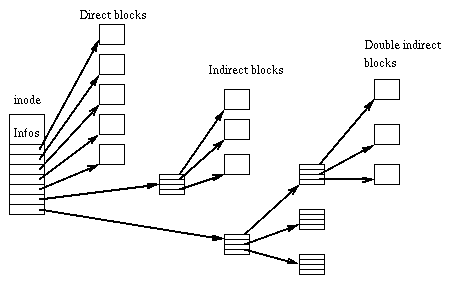
\includegraphics{./images/Ext2-inode.png}
 % Ext2-inode.png: 456x286 pixel, 96dpi, 12.06x7.57 cm, bb=0 0 342 214
\end{center}


\subsubsection{Block Groups}
En busqueda de eficiencia y organizacion, ext2 divide los bloques de la particion en varios grupos.
Estos grupos tienen un numero igual de bloques y de inodes.

El objetivo principal de creacion de estos, es reducir la fragmentacion. 
Permiten buscar bloques disponibles para uso dentro del mismo grupo en el que se encuentra un inode, asi teniendo toda la informacion en bloques lo mas cercanos posibles.

En particular, estos contienen:
\begin{itemize}
\item Bitmap de uso de bloques
\item Bitmap de uso de inodes
\item Tabla de inodes
\item Bloques de datos
\end{itemize}

La ubicacion de esta informacion, y otros datos sobre el uso de un dado grupo, se encuentra en la \textit{Block Group Descriptor Table}.
Esta se encuentra en el bloque inmediatamente posterior al \textit{Superblock}.
En ella se almacenan muchos datos utilizados con el objetivo de poder verificar el correcto estado del file system.

\subsubsection{Entradas de directorio}
ext2 define como se almacena el contenido de un directorio.
Se hace de una manera muy simple en forma de \textit{Linked List}.
Cada entrada contiene un nombre, y un numero de inode al que hace referencia.
Como consecuencia, cada inode puede ser referencia con mas de un nombre, creando lo conocido como \textit{hard links}.

\subsubsection{Limitaciones}
El tamaño maximo de la particion, y de los inodes, es definido en funcion del tamaño de bloque.
Y en nuestro caso, se ve limitado por el driver ATA que soporta direccionar hasta $ 2^{28} $ sectores.

El limite teorico de tamaño total viene dado por $ 2^{32} * blockSize $.
Ahora, como nuestro driver ATA soporta solo sectores de 512 bytes, el limite real es $ 2^{28} * 512 bytes $.

El limite de tamaño de un inode viene dado por:
$$( \frac{blockSize}{4}^3 + \frac{blockSize}{4}^2 + \frac{blockSize}{4} + 11 ) * blockSize $$

\subsubsection{Cache}
Dado lo caras que son las operaciones a disco, y la limitacion de poder trabajar de a sectores, el FS tiene una serie de buffers que usa para mitigar estos efectos.
Estos permiten por ejemplo, mantener cargados entre operaciones los indices de un inode.
O hacer escrituras parciales sin preocupaciones.
Si bien el diseño ideal utiliza un cache de tamaño dinamico, por simplicidad optamos por una cantidad fija de buffers manejada internamente por el FS.

\subsection{Virtual file system}

Para proveer una interfaz desacoplada de la implementacion particular de ext2, creamos el \textit{VFS}.
Este representa en memoria la estructura de inode y \textit{File Descriptors}.
Y es el que utilizan los procesos para leer y escribir de archivos.

Este diseño nos permitio gran flexibilidad a la hora de implementar los distintos comportamientos esperados del file system.

\subsection{Apertura y manejo de archivos}
En una primera instancia nos encargamos de adaptar nuestras llamadas a sistema y nuestra librería estandar
para que puedan desarrollar las nuevas funcionalidades de nuestro sistema operativo.
Las llamadas a \textit{read} y \textit{write} podían ahora escribir en archivos, así como las llamadas a \textit{open} y \textit{close} se hicieron
necesarias cuando antes no lo fueron.
Al hacer una llamada a \textit{open()}, esta actualizaba tanto a nivel kernel como a nivel proceso que cierto archivo habia sido abierto. 
Como ya fue dicho, un proceso contaba con una tabla de \textit{file descriptors}. 
Estos, apuntan al \textit{inode} siendo manipulado y además cuentan con punteros a función que indican como deben comportarse lecturas y escrituras (entre otras cosas) dependiendo el tipo de archivo 
(podría bien ser un archivo regular o un link simbolico por ejemplo). 
Esto permitió que las implementaciones de \textit{read()}, \textit{write()} y \textit{close()} sean bastante sencillas. 
    
Estas llamadas a sistema fueron siendo extendidas a medida que la funcionalidad del sistema operativo crecía. 
Como será visto en las proximas secciones, se escribieron funciones adecuadas para la manipulación de cada tipo de archivo.

\subsection{Tabla de inodes}
Para evitar tener duplicada informacion en memoria, creamos una tabla de inodes abiertos.
Esta tabla es consultada antes de hacer cualquier busqueda en disco, e implementa un sistema simple de \textit{Reference Counting}.

\subsection{Directorios}

Ya a bajo nivel era posible detectar el tipo de \textit{inode} guardado en el sistema. Un directorio simplemente era
un inode que en su contenido se guardan referencias hacía otros inodes. Tanto la interfaz del driver Ext2 como la del
vfs permiten escribir directorios de forma correcta. Cabe destacar que ademas de la referencia al inode, una entrada
de directorio también guarda el nombre de la entrada que luego verá el usuario.

\subsection{FIFO}
La implementacion de \textit{FIFOs} resulto trivial, ya que muchas de las decisiones diseño tomadas antes de implementarlos los tenian en cuenta.
La existencia de la estructura \textit{FileDescriptorOps} que contiene punteros a funcion con las operaciones realizables sobre un File Descriptor, permitio que la implementacion sea totalmente transparente a nivel sistema.

Al inode que representa un FIFO, cuando es abierto por primera vez se le asocia una estructura \textit{FIFO}.
Como todos los File Descriptors que representan un mismo archivo hacen referencia al mismo inode, todos tiene acceso la estructura \textit{FIFO}.
Esta contiene el buffer donde se guardan los datos escritos al FIFO, cuantos procesos abrieron el fifo, y otro datos utiles.

Cabe destacar el comportamiento de los FIFOs en cuanto su apertura, estrictura y lectura.
Cuando se abre un FIFO, el proceso se bloquea hasta que el FIFO es abierto por al menos un proceso para lectura, y otro para escritura.
La lectura de un FIFO es bloqueante, es decir si no hay contenido para leer el proceso bloquea hasta que lo haya.
De la misma manera, la escritura es bloqueante en caso de que el FIFO no tenga espacio para escribir los datos.

En caso de que alguna punta del FIFO sea cerrada por todos los procesos que la abrieron, cualquier operacion en curso se cancela, y retorna que se procesaron 0 bytes.

\subsection{Links simbolicos}
La implementación de links simbolicos implicaba la creación de nodos que inclusive en el sistema Ext2 eran marcados
como links simbolicos. El contenido de los mismos simplemente indicaba el \textit{path} del archivo al que este
hacia referencia.
Luego, a la hora de leer un archivo que sea un link simbolico (o al tratar de resolver un \textit{path} cuyo alguno
de sus directorios era un link simbolico) bastaba con reemplazar el este archivo con el link al que realmente
apuntaba.

En esta implementación (al igual que en el resto) tratamos de ser lo más fieles al entorno \textit{UNIX} como 
era posible.

\subsection{Character devices}
Para nuestra implementacion de \textit{tty}, usamos el tipo especial de archivos \textit{Character device}.
Esto quiere decir que toda la comunicacion entre la terminal y los procesos corriendo en ella, pasan atravez del \textit{VFS}.

\subsection{Current working directory}
    
Como ya fue mencionado, cada proceso contiene información sobre cual era el \textit{current working directory} en
el momento en que fue ejecutado. Esto permite que la obtención del \textit{current working directory} sea sencilla
y manipulable en los momentos necesarios, sobre todo para permitir \textit{paths} relativos.

    
\subsection{Permisos del sistema}
Una vez implementados usuarios y grupos era fácil saber el gid y el uid de un proceso. Dada la forma en que estaba
implementado nuestro \textit{file system}, Ext2 contaba con lugares especificos para guardar tanto los permisos y el
uid y gid del archivo. Además, las prestaciones del vfs hacían que estos datos también fuesen fáciles de obtener.

Una vez conseguidos estos datos, era trivial evaluar en que casos se permitía abrir un archivo, teniendo en cuenta
que tanto el archivo tenga los permisos adecuados así como el \textit{path} que lo contiene.

\newpage
\section{Comandos provistos}
Para poder probar y mostrar las nuevas funcionalidades del trabajo hubo que agregar ciertos comandos y funcionalidades ejecutables desde la consola. 
La lista completa de comandos disponibles puede encontrarse mediante el comando \textit{help}, y la documentacion de cada comando mediante el comando \textit{man}.
A continuación se presentan algunos casos interesantes.

\newpage
\section{Agregados}
\subsection{Memory managment}
Inicialmente, el TP contaba con multiples arrays de tamaño estatico para guardar todos los datos internos del kernel.
Por supuesto, esta solucion es menos que optima, ya que genera un desperdicio de memoria e impone limites arbitrarios al sistema.
Para evitar esto, desarrollamos un sistema de allocacion de paginas de memoria.
Y encima de este sistema, utilizamos la implementacion de \textit{malloc} de Dario Sneidermanis, publicada en \href{https://github.com/esneider/malloc}{Github}.

Para allocar paginas, hicimos uso de informacion provista por \textit{Grub} que permite saber que zonas de memoria se pueden utilizar, y cuanta memoria hay disponible.
Esta memoria la dividimos en bloques de $4KB$, teniendo en mente la posibilidad de agregar paginacion al sistema.
Para obtener estas paginas optamos por un simple algoritmo de allocacion basado en un bitmap de uso de paginas.

Una caracteristica interesante de la implementacion de \textit{malloc}, es que permite tener varios contextos de memoria distintos.
Lo que facilito tener un contexto de memoria para el kernel, y otro para cada proceso (excepto los procesos de kernel que usan el mismo que el kernel).
La unica limitacion del sistema es que los contextos de proceso tienen un tamaño fijo, mientras que el del kernel crece a medida que es necesario.

\subsection{Terminal control sequences}
Nuestra implementacion de terminal soporta una gran parte de \href{http://invisible-island.net/xterm/ctlseqs/ctlseqs.html}{xterm control sequences}.
Estas permiten manipular el cursor y el color de la pantalla desde los procesos utilizando solo la primitiva \textit{write}.

\newpage
\section{Problemas encontrados}

Durante el desarrollo de este trabajo practico fueron surgiendo diferentes dudas y problemas. El proposito de esta
sección es comentarlos con el fin del aprendizaje.

Un dilema bastante frecuente a lo largo del trabajo practico es lo que nos gusta llamar "gallina o huevo". Al realizar
un desarrollo a bajo nivel que ha comenzado con pocos recursos, era habitual encontrarse con la duda de si convenía
arrancar a implementar la lectura o la escritura de alguna prestación. Es evidente que si se hacía primero la lectura, 
no había forma de probar su funcionamiento ya que no existía la escritura. Lo mismo sucedía a modo inverso. Si bien 
la solución no era complicada (desarrollar todo) era incomodo y molesto a la hora de encontrar errores ya que los mismos
podían encontrarse en cualquier lado.

Varios problemas interesantes surgieron durante la creación del \textit{driver} ATA. A pesar de que se siguieron
rigurosamente los estándares, se encontró que no todos los emuladores funcionaban de forma correcta con el mismo.
Inclusive, detectamos que el driver no se comportaba de manera deseada al tratar con varios sectores a la vez con lo
cual nos vimos forzados a modificar la lógica interna del driver simulando un acceso a multiples sectores a tráves de
varios accesos de a un sector a la vez.


<<<< Mencionar el tema de los comandos internos de la shell >>>>

\newpage     
\section{Referencias}

\begin{itemize}
  \item Material provisto por la cátedra
  \item The C programming language - Kernighan y Ritchie
  \item http://invisible-island.net/xterm/ctlseqs/ctlseqs.html
  \item http://webpages.charter.net/danrollins/techhelp/0087.HTM
  \item http://faydoc.tripod.com/cpu/rdtsc.htm
  \item http://stanislavs.org/helppc/
  \item http://www.linux.it/~rubini/docs/ksys/ksys.html
  \item http://wiki.osdev.org
  \item http://wiki.osdev.org/Detecting\_CPU\_Speed
  \item	http://wiki.osdev.org/CMOS\#Accessing\_CMOS\_Registers
  \item http://wiki.osdev.org/Bootable\_CD
  \item http://wiki.osdev.org/Boot\_sequence\#Easy\_Way\_Out
  \item http://wiki.osdev.org/Ext2
  \item http://wiki.osdev.org/IDE
  \item http://wiki.osdev.org/ATA\_PIO\_Mode
  \item http://en.wikipedia.org/wiki/System\_time\#Retrieving\_system\_time
  \item http://en.wikipedia.org/wiki/Calculating\_the\_day\_of\_the\_week
  \item http://cplusplus.com/
  \item http://github.com/esneider/malloc
  \item http://www.nongnu.org/ext2-doc/ext2.html
\end{itemize}
   
\end{document}
